\documentclass[10pt,twocolumn,letterpaper]{article}

\usepackage{cvpr}
\usepackage{times}
\usepackage{epsfig}
\usepackage{graphicx}
\usepackage{amsmath}
\usepackage{amssymb}
% Include other packages here, before hyperref.

% If you comment hyperref and then uncomment it, you should delete
% egpaper.aux before re-running latex.  (Or just hit 'q' on the first latex
% run, let it finish, and you should be clear).
%\usepackage[breaklinks=true,bookmarks=false]{hyperref}

\cvprfinalcopy % *** Uncomment this line for the final submission

\def\cvprPaperID{****} % *** Enter the CVPR Paper ID here
\def\httilde{\mbox{\tt\raisebox{-.5ex}{\symbol{126}}}}
% Pages are numbered in submission mode, and unnumbered in camera-ready
%\ifcvprfinal\pagestyle{empty}\fi
\setcounter{page}{1}
\begin{document}

%%%%%%%%% TITLE
\title{Freddie Mac Final Report}

\author{Thomas Billman}
% For a paper whose authors are all at the same institution,
% omit the following lines up until the closing ``}''.
% Additional authors and addresses can be added with ``\and'',
% just like the second author.
% To save space, use either the email address or home page, not both

\maketitle
%\thispagestyle{empty}

%%%%%%%%% ABSTRACT

%%%%%%%%% BODY TEXT
%Project 1 Text
\section{Introduction}

Freddie Mac holds a large portion of the United States of America's home mortgages. As such looking for trends in the values and performance of these loans is crucial. Our dataset consists of data collected at the time loans were issued and a calculated Net Present Value (NPV) that acts as a proxy for the total value of each loan. This paper summarizes a subset of the different variables found in the dataset. The dataset can be found on my GitHub at the following address:
https://tinyurl.com/ycpr8lrj

%-------------------------------------------------------------------------
\section{Variables}
\subsection{Credit Score}

Figure \ref{fig:CreditScoreSummary} shows us the summary statistics of Credit Score, and Figure \ref{fig:CreditScoreHist} shows us the distribution. This distribution is skewed left with many individuals in the 650 - 775 range. 

\subsection{First Payment}

Figure \ref{fig:FirstPaymentS} shows us the frequency table of the year and month the first payment was made for each loan.Figure \ref{fig:FirstPaymentB} shows us the distribution as a bar chart. This distribution shows us that most borrowers made their first payment in the first half of 1999 with a few outliers all the way out into 2004.

\subsection{First Time Home Buyer Flag}

Figure \ref{fig:FirstTimeHomeS} shows us the frequency table of the flag marking if the borrowers for each loan were first time home buyers. This shows that very few (~10\%) of the loans were from these borrowers. Another notable quality is the amount of unreported data (~33\%). Figure \ref{fig:FirstTimeHomeB} shows us the distribution as a bar chart. This shows the same data as the summary. 

\subsection{Loan Maturity Date}

Figure \ref{fig:MaturityS} shows us the frequency table of the date the loans will mature or end. This shows a large spike in early 2029, which would be 30 years from most of the loans' origination date. This makes sense, and like the previous variable we also have some outliers sprinkled around the surrounding years. Figure \ref{fig:FirstTimeHomeB} shows us the distribution as a bar chart. This shows the same data as the summary. 

\subsection{Metropolitan Statistical Area (MSA) Codes}

Figure \ref{fig:MSAS} shows us the frequency table of the MSA codes of these homes. The actual codes do not give a lot of pertinent information, but we can not the large count of those marked Other and NA. "Other" likely refers to rural homes not included in an MSA. Figure \ref{fig:MSAB} shows us the distribution as a bar chart. This shows the same data as the summary. 

\subsection{Mortgage Insurance Percentage}

Figure \ref{fig:MIS} shows us the summary statistics of the mortgage insurance percentages of the homes. It is interesting to note that the majority of homes do not require mortgage insurance and the large amount of underreporting. Figure \ref{fig:MIB} shows us the distribution as a histogram. This also shows us that the majority of mortgage insurance policies are in round percentages(10\%, 25\%, etc.).

\subsection{Number of Units}

Figure \ref{fig:MIS} shows us the summary statistics of the number of units each loan covers. It is interesting to note that the vast majority of loans cover just one loan, however there are some that go as high as covering four units. It is also worth noting that in this case there are very few NAs. Figure \ref{fig:MIB} shows us the distribution as a bar chart. 

\subsection{Occupancy Status}

Figure \ref{fig:OccS} shows us the frequency table of the occupancy status of each home. This shows that the vast majority of these homes are owner occupied, while there is a subset that are either investments or secondary homes. Figure \ref{fig:OccB} shows us the distribution as a bar chart. 

\subsection{Combined Loan to Value}

Figure \ref{fig:CLTVS} shows us the Combined Loan to Value Ratio of each home. This is the initial loan amount plus any lent to refinance divided by the cost of the home. This shows that most loans have a CLTV of around 80\%. Figure \ref{fig:CLTVB} shows us the distribution as a histogram. This shows us that many people try to get as close to 80\% as they can without going over. Usually going over requires mortgage insurance, which many borrowers prefer not to pay.

\subsection{Debt to Income Ratio}

Figure \ref{fig:DTIS} shows us the summary statistics of the Debt to Income Ratio of each loan. This is the percent of the borrower's income each month that is paid to the mortgage. Most of the data is in the 20-40\% range. Figure \ref{fig:DTIB} shows us the distribution as a histogram. This distribution is surprisingly very normal.

\subsection{Unpaid Balance}

Figure \ref{fig:UPBS} shows us the summary statistics of the initial unpaid balances of each loan. This is the same thing as the amount loaned. This shows that most loans at this time were around \$100,000. Figure \ref{fig:UPBB} shows us the distribution as a histogram. It is interesting that there is a sharp decrease around \$250,000. This is because Freddie Mac generally does not accept loans with balances over \$250,000.

\subsection{Interest Rate}

Figure \ref{fig:IRS} shows us the summary statistics of the interest rate of each loan. At this time most interest rates were around 6-7\%. Figure \ref{fig:IRB} shows us the distribution as a histogram. 

\subsection{Property Type}

Figure \ref{fig:PTS} shows us the frequency table of the property type of each home. This shows that the majority of the loans are for single family homes, planned units, and condominiums. Figure \ref{fig:PTB} shows us the distribution as a bar chart. 

\subsection{Number of Borrowers}

Figure \ref{fig:NOBS} shows us the summary statistics of the number of borrowers on each loan. This shows that the majority of loans actually have two borrowers. Figure \ref{fig:NOBB} shows us the distribution as a bar chart. 

\subsection{Net Present Value (NPV)}

Figure \ref{fig:NPVS} shows us the summary statistics of the NPV of each loan. The NPV is our proxy of how profitable a loan ended up being for the lender. This shows that most loans end up netting the lender around \$10,000 - \$20,000 over what a 30 year government bond would yield. Figure \ref{fig:NPVB} shows us the distribution as a histogram. This shows the high volatility associated with the NPVs of these loans. Additionally how far out the outlying data points are. 

% Project 2 Text

\section{Linear Regression}
\subsection{Simple Linear}
We begin our analysis with a simple linear regression using all the variables our dataset provides to us. Two variables have been removed due to a lack of contrast. These columns only contained one value so they are not useful for prediction. Additional categorical variables such as zip code and MSA code were removed due to a high number of insignificant dummy variables being produced. The resulting summary of our first linear regression can be found in Figure \ref{fig:lm1s}. This shows that some of our variables have very little impact on predicting NPV. Particularly the number of borrowers associated with the loan. The introduction of a second borrower was only shown to lower the value of the NPV by around 11 cents which is very insignificant. However, were many variables that showed correlations that were very statistically significant. However, our $R^2_a$ value is very low at only .01026. Additionally the residual plots found in Figure \ref{fig:lm1c} show strong heteroscedasticity in our dataset particularly around the mean. In an attempt to boost predictive power we look to remove some variables. 

\subsection{Variable Reduction}

We begin a simple variable reduction by removing variables that are not statistically significant in our first regression. A summary of this regression can be shown in Figure \ref{fig:lm2s} and the residual plots can be found in Figure \ref{fig:lm2c}. This summary shows that our $R^2_a$ value actually decreased and our residual plots look largely the same. However, this should be useful for the next step where we check for interactions between these variables.

\subsection{Interaction Terms}
Due to screen size limitations Figure \ref{fig:lm3s} does not show all variables included in the regression, however the $R^2_a$ value jumped to .01152. Other interesting finds were that variables that were previously significant such as Credit Score now become insignificant as most of the predictive power was wrapped up in interactions with other variables in the dataset. Again, the residuals shows in Figure \ref{fig:lm3c} show similar trends to the previous residual plots. These models show that there is a lot of discretion available for variable selection when creating a linear model for this dataset. Although this is not a comprehensive review, it provides a good baseline to build upon with more advanced statistical techniques.

%Project 3 Text
\section{Logistic Regression}
We begin our further analysis by predicting whether the NPV of an observation will be positive or negative. The covariates considered include Credit Score, Mortgage Insurance, Debt to Income ratio, among others. This model predicted that every mortgage would have a positive NPV, so it's accuracy measures were as follows:
\begin{center}
	\begin{tabular}{ |c|c| } 
		\hline
		Sensitivity & 1 \\ 
		\hline
		Specificity & 0 \\
		\hline
		Accuracy & 0.98125\\ 
		\hline
	\end{tabular}
\end{center}

Additionally the ROC Curve can be found in Figure \ref{fig:ROC}. The area under the curve was .6417, which is not very significant.

\section{Linear Discriminant Analysis}

We continue by applying Linear Discriminant Analysis. These results were the same as logistic regression, by predicting all rows as positive NPV. 
\begin{center}
	\begin{tabular}{ |c|c| } 
		\hline
		Sensitivity & 1 \\ 
		\hline
		Specificity & 0 \\
		\hline
		Accuracy & 0.98125\\ 
		\hline
	\end{tabular}
\end{center}

\section{Quadratic Discriminant Analysis}

Quadratic Discriminant Analysis begins predicting NPVs that are not all positive. The table of results is as follows:

\begin{center}
	\begin{tabular}{ |c|c|c| } 
		\hline
		& True - & True +\\ 
		\hline
		Predicted - & 246 & 1587 \\ 
		\hline
		Predicted + & 3676 & 203619\\
		\hline
	\end{tabular}
\end{center}

This yields the following sensitivity, specificity, and accuracy:
\begin{center}
	\begin{tabular}{ |c|c| } 
		\hline
		Sensitivity & 0.9922663 \\ 
		\hline
		Specificity & 0.0627231 \\
		\hline
		Accuracy & 0.9748336\\ 
		\hline
	\end{tabular}
\end{center}

It is worth noting that although a specificity of .06 seems poor, it is nearly 3 times more accurate than random guessing.


\section{KNN Analysis}

We continue through to KNN analysis, which produced even better specificity than QDA. This was the resulting confusion matrix:

\begin{center}
	\begin{tabular}{ |c|c|c| } 
		\hline
		& True - & True +\\ 
		\hline
		Predicted - & 601 & 209 \\ 
		\hline
		Predicted + & 3321 & 204997\\
		\hline
	\end{tabular}
\end{center}
This yields the following sensitivity, specificity, and accuracy:
\begin{center}
	\begin{tabular}{ |c|c| } 
		\hline
		Sensitivity & 0.1532381 \\ 
		\hline
		Specificity & 0.9989815 \\
		\hline
		Accuracy & 0.9831204 \\ 
		\hline
	\end{tabular}
\end{center}

Of the four methods tested this had the best accuracy and impressive specificity for this dataset. 


\section{Cross Validated Results}

We repeat the above methods using 5-fold cross validation.

\subsection{Logistic Regression}
Overall average accuracy was 0.981719 and took ~15 seconds to run. All sensitivities were 1 and all specificities were 0.

\subsection{LDA Analysis}
Overall average accuracy was 0.9812459  and took ~5 seconds to run. All sensitivities were 1 and all specificities were 0.

\subsection{QDA Analysis}
Overall average accuracy was 0.9747953 and took ~ 4 seconds to run. All sensitivities were ~ .992 and specificities were between .049 and .075.

\subsection{KNN Analysis}
Overall average accuracy was 0.9806004 and took ~ 9 minutes to run. All sensitivities were ~ .998 and specificities were between .077 and .087.


\section{Recap}
These models show that QDA and KNN were better classifiers for our data than logistic or LDA. Additionally, cross validated results show lower accuracies than testing on your training data. However, this is to be expected.


%-------------------------------------------------------------------------

%Project 4 Text

\section{KNN Selection of K}
We begin this project by testing different values of K for accuracy. For this I decided to use 5-fold cross validation in order to evaluate choices of K by testing accuracy rather than training accuracy. I tested values of 1,3,5,7,9, and 11.
\begin{center}
	\begin{tabular}{ |c|c| } 
		\hline
		K & Accuracy \\ 
		\hline
		1 & 0.9806052 \\
		\hline
		3 & 0.9806052\\ 
		\hline
		5 & 0.9806195\\ 
		\hline
		7 & 0.98061\\ 
		\hline
		9 & 0.98061\\ 
		\hline
		11 & 0.98061\\ 
		\hline
	\end{tabular}
\end{center}

This code took 37 minutes to run. This shows that all choices of K amongst this set have essentially identical accuracies. We will continue this analysis using K = 3.

\section{5-Fold Cross Validation}

In this section we apply 5-fold cross validation to the Logistic, LDA, QDA, and KNN models previously selected.

\begin{center}
	\begin{tabular}{ |c|c|c|c|c| } 
		\hline
		Model & Acc & Sens & Spec & Run Time\\ 
		\hline
		Logistic & 0.9812 & 1 & 0 & 10 s \\
		\hline
		LDA & 0.9812 & 1 & 0 & 4.7 s\\ 
		\hline
		QDA & 0.9747 & 0.9922 & 0.06339 & 4.2 s\\ 
		\hline
		KNN & 0.9806 & 0.9978 & 0.08076 & 6.5 m\\ 
		\hline
		
	\end{tabular}
\end{center}

This shows that Logistic and LDA predicted all observations as positive NPV to achieve the greatest overall accuracy. However, I would pick KNN as a model given that it can predict negative NPVs at a value over four times their relative occurrence in the population. Additionally, the accuracies for these models can be found in Figure \ref{fig:5f}



\section{Leave-One-Out Cross Validation (LOOCV)}

We continue this cross validation by utilizing LOOCV. This is the least biased as it does not involve any randomization. However, it is also the most computationally intensive. Due to our large dataset it was necessary to utilize parallel computation techniques and High Performance Computing resources. The results of our LOOCV were as follows:

\begin{center}
	\begin{tabular}{ |c|c|c|c|c| } 
		\hline
		Model & Acc & Sens & Spec & Time to Run  \\ 
		\hline
		Logistic & 0.9812 & 1 & 0 & 1.1 days \\
		\hline
		LDA & 0.9812 & 1 & 0 & 7.5 hours\\ 
		\hline
		QDA & 0.9748 & 0.9922 & 0.07503 & 6.6 hours\\ 
		\hline
		KNN & 0.9805 & 0.9972 & 0.09778 & 26 minutes\\ 
		\hline
		
	\end{tabular}
\end{center}

It is also worth noting that any boxplots for these accuracies would be degenerate as accuracies in LOOCV can only take values of 1 or 0. Due to this lack of interpretation, they are not included in this paper.These models show that KNN was our best classifier for our data, particularly when utilizing LOOCV. 

\section{Random Forest}
Near the end of this course, we learned about Random Forest classification and regression. This method involves randomly selecting subsets of your covariates and training decision trees. After training 500 trees, a majority vote or average vote is taken.

\subsection{Classification}
 By applying this technique to our dataset and using 5-fold cross validation, we derived the following results:
 
\begin{center}
	\begin{tabular}{ |c|c|c|c| } 
		\hline
		Fold & Acc & Sens & Spec   \\ 
		\hline
		1 & 0.9801 & 0.9988 & 0.1700 \\
		\hline
		2 & 0.9837 & 0.9987 & 0.1551 \\ 
		\hline
		3 & 0.9822 & 0.9988 & 0.1330 \\ 
		\hline
		4 & 0.9840 & 0.9987 & 0.1489 \\ 
		\hline
		5 & 0.9845 & 0.9992 & 0.1436 \\ 
		\hline
		
	\end{tabular}
\end{center}

This gives us an average accuracy similar to our other classifiers, however it is very notable that Random Forest classification can pick out loans with negative NPVs at a rate nearly ten times their rate of occurrence in the data set. This makes it the best classifier out of all that we have considered. We can compare Random Forest accuracy to our other classification methods in Figure \ref{fig:RF}

\subsection{Regression}

By applying this method to estimate NPV as a continuous variable we get the following results:

\begin{center}
	\begin{tabular}{ |c|c| } 
		\hline
		Fold & Testing $R^2$    \\ 
		\hline
		1 & .019  \\
		\hline
		2 & .0208  \\ 
		\hline
		3 & .0201  \\ 
		\hline
		4 & .0173  \\ 
		\hline
		5 & .0205  \\ 
		\hline
		
	\end{tabular}
\end{center}

This gives us a mean $R^2$ of .0195. This explains nearly twice the variance of the dataset compared to our reduced variable linear model, however still provides very little insight into our dataset.


\section{Conclusion}
Although it would be nice to be able to consistently predict what the value of a loan would be at the time of origination, there seems to be too much that goes into whether or not a borrower defaults. An individual's credit score and income can not predict whether the borrower will lose their job some time in the next 30 years. By adding micro and macroeconomic data and collating additional quarters of loan data, we may improve predictive power in the future.

\section{References}
A. Liaw and M. Wiener (2002). Classication and Regression by randomForest. R News 2(3), 18{22}.

Breiman, Leo. "Random forests." Machine learning 45.1 (2001): 5-32.	

Deng, Grace. "Analyzing the Risk of Mortgage Default" (2016)	

Freddie Mac. “Single Family Loan-Level Dataset General User Guide”: http://www.freddiemac.com/research/pdf/user\textunderscore guide.pdf
	
Kutner, Michael H. Applied linear regression models. {4th ed}. Michael H. Kutner, Christopher J. Nachtsheim, John Neter.

%Project 1 Figures

%Credit Score
\begin{figure}
	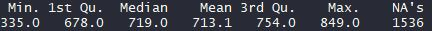
\includegraphics[width=0.45\textwidth]{images/CreditScoreSummary.JPG}
	\caption{Summary Statistics of Credit Score}
	\label{fig:CreditScoreSummary}
\end{figure}
\begin{figure}
	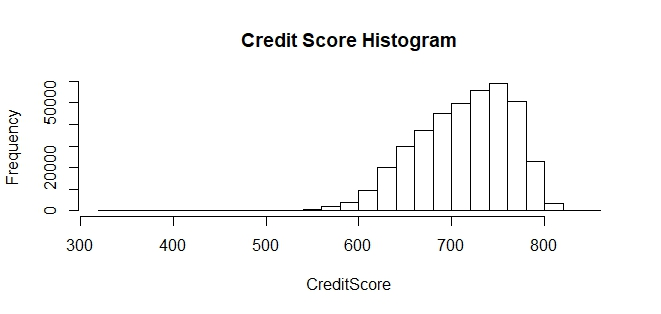
\includegraphics[width=0.45\textwidth]{images/CreditScoreHist.jpeg}
	\caption{Histogram of Credit Score}
	\label{fig:CreditScoreHist}
\end{figure}

%First Payment
\begin{figure}
	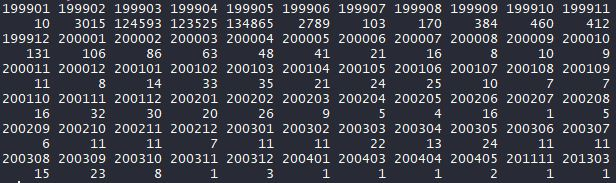
\includegraphics[width=0.45\textwidth]{images/FirstPaymentSummary.JPG}
	\caption{Frequency Table of First Payment}
	\label{fig:FirstPaymentS}
\end{figure}
\begin{figure}
	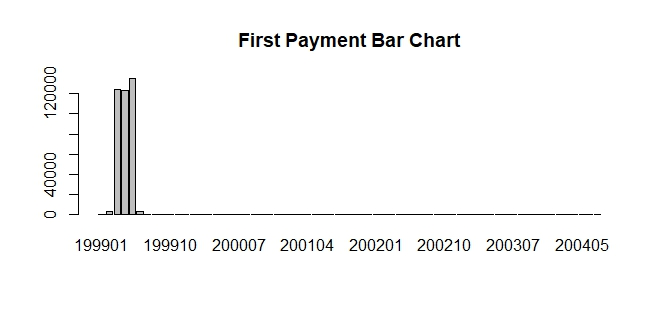
\includegraphics[width=0.45\textwidth]{images/FirstPaymentBarChart.jpeg}
	\caption{Histogram of Credit Score}
	\label{fig:FirstPaymentB}
\end{figure}

%FirstTimeHome
\begin{figure}
	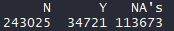
\includegraphics[width=0.45\textwidth]{images/FirstTimeHomeS.JPG}
	\caption{Frequency Table of First Time Home Buyers}
	\label{fig:FirstTimeHomeS}
\end{figure}
\begin{figure}
	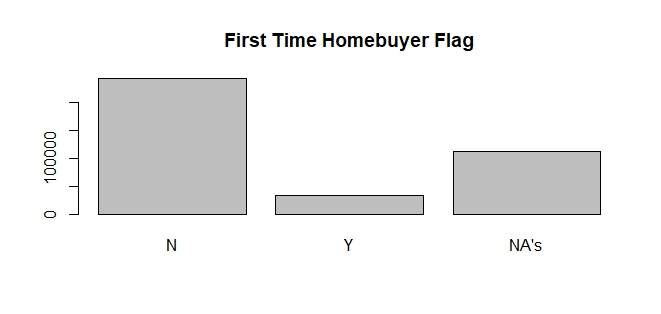
\includegraphics[width=0.45\textwidth]{images/FirstTimeHomeB.jpeg}
	\caption{Bar Chart of First Time Home Buyer Flag}
	\label{fig:FirstTimeHomeB}
\end{figure}

%Maturity
\begin{figure}
	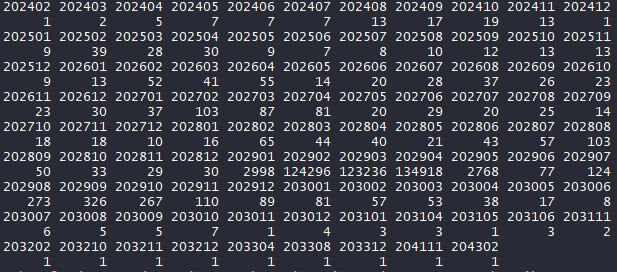
\includegraphics[width=0.45\textwidth]{images/MaturityS.JPG}
	\caption{Frequency Table of loan maturity date}
	\label{fig:MaturityS}
\end{figure}
\begin{figure}
	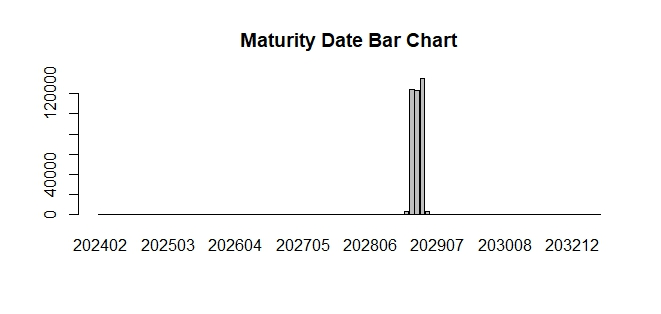
\includegraphics[width=0.45\textwidth]{images/MaturityB.jpeg}
	\caption{Bar Chart of loan maturity date}
	\label{fig:MaturityB}
\end{figure}

%MSA
\begin{figure}
	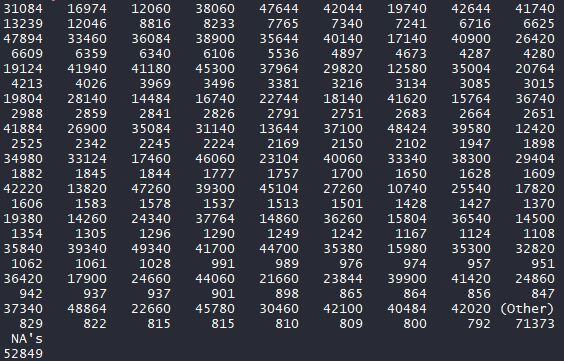
\includegraphics[width=0.45\textwidth]{images/MSAS.JPG}
	\caption{Frequency Table of Metropolitan Statistical Area locations}
	\label{fig:MSAS}
\end{figure}
\begin{figure}
	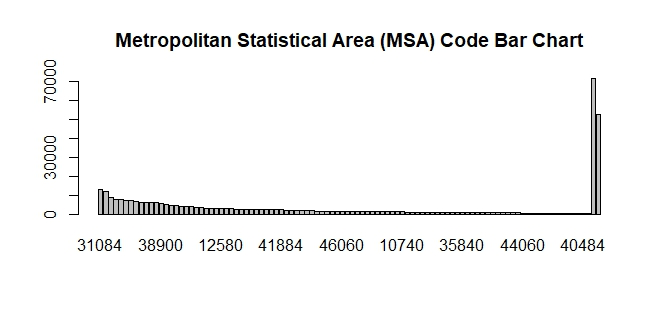
\includegraphics[width=0.45\textwidth]{images/MSAB.jpeg}
	\caption{Bar Chart of Metropolitan Statistical Area locations}
	\label{fig:MSAB}
\end{figure}

%MI
\begin{figure}
	\includegraphics[width=0.45\textwidth]{images/MIS.JPG}
	\caption{Summary Statistics of Mortgage Insurance Percentage}
	\label{fig:MIS}
\end{figure}
\begin{figure}
	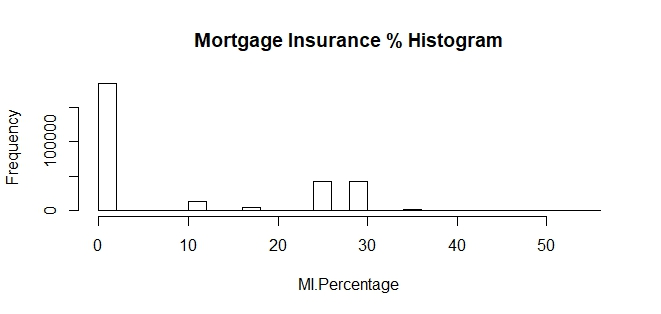
\includegraphics[width=0.45\textwidth]{images/MIB.jpeg}
	\caption{Bar Chart of Mortgage Insurance Percentage}
	\label{fig:MIB}
\end{figure}

%NOU
\begin{figure}
	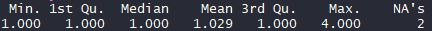
\includegraphics[width=0.45\textwidth]{images/NOUS.JPG}
	\caption{Frequency Table of Number of Units}
	\label{fig:NOUS}
\end{figure}
\begin{figure}
	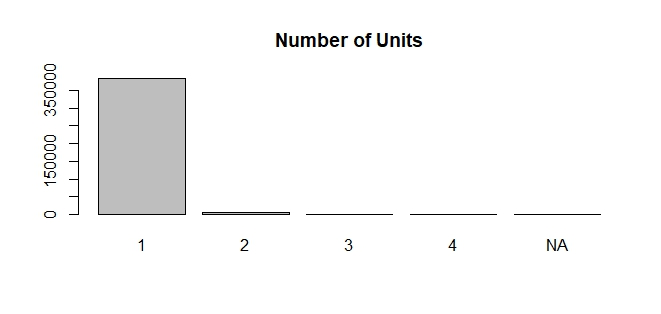
\includegraphics[width=0.45\textwidth]{images/NOUB.jpeg}
	\caption{Bar Chart of Number of Units}
	\label{fig:NOUB}
\end{figure}

%Occ
\begin{figure}
	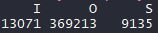
\includegraphics[width=0.45\textwidth]{images/OccS.JPG}
	\caption{Frequency Table of Occupancy Status}
	\label{fig:OccS}
\end{figure}
\begin{figure}
	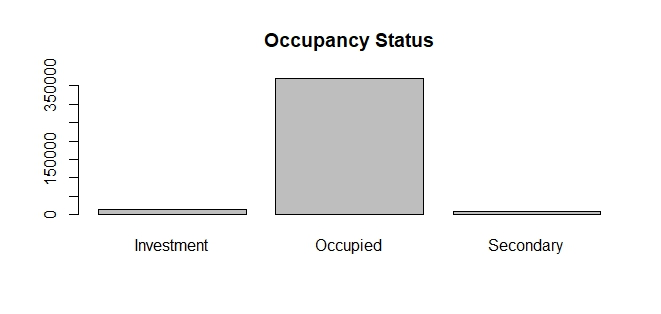
\includegraphics[width=0.45\textwidth]{images/OccB.jpeg}
	\caption{Bar Chart of Occupancy Status}
	\label{fig:OccB}
\end{figure}

%CLTV
\begin{figure}
	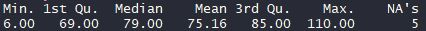
\includegraphics[width=0.45\textwidth]{images/CLTVS.JPG}
	\caption{Summary Statistics of Combined Loan to Value Ratio}
	\label{fig:CLTVS}
\end{figure}
\begin{figure}
	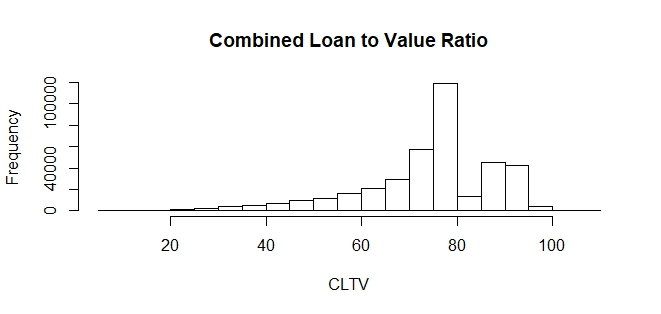
\includegraphics[width=0.45\textwidth]{images/CLTVB.jpeg}
	\caption{Histogram of Combined Loan to Value Ratio}
	\label{fig:CLTVB}
\end{figure}

%DTI
\begin{figure}
	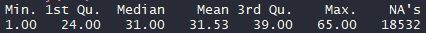
\includegraphics[width=0.45\textwidth]{images/DTIS.JPG}
	\caption{Summary Statistics of Debt to Income Ratio}
	\label{fig:DTIS}
\end{figure}
\begin{figure}
	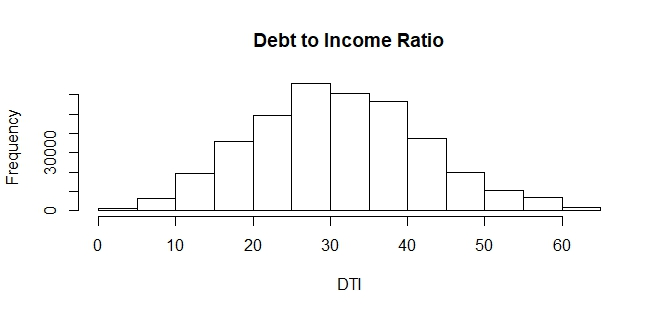
\includegraphics[width=0.45\textwidth]{images/DTIB.jpeg}
	\caption{Histogram of Debt to Income Ratio}
	\label{fig:DTIB}
\end{figure}

%UPB
\begin{figure}
	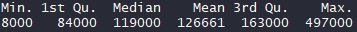
\includegraphics[width=0.45\textwidth]{images/UPBS.JPG}
	\caption{Summary Statistics of Unpaid Balance}
	\label{fig:UPBS}
\end{figure}
\begin{figure}
	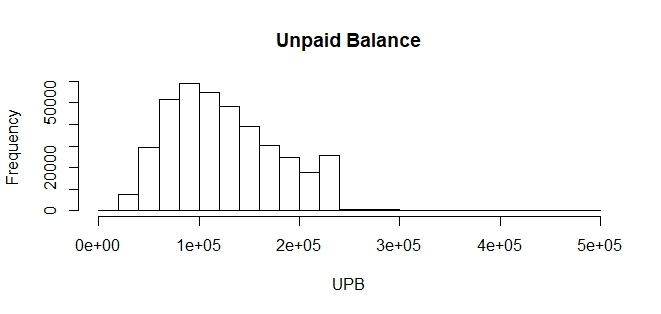
\includegraphics[width=0.45\textwidth]{images/UPBB.jpeg}
	\caption{Histogram of Unpaid Balance}
	\label{fig:UPBB}
\end{figure}

%IR
\begin{figure}
	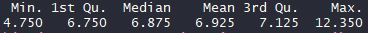
\includegraphics[width=0.45\textwidth]{images/IRS.JPG}
	\caption{Summary Statistics of Interest Rate}
	\label{fig:IRS}
\end{figure}
\begin{figure}
	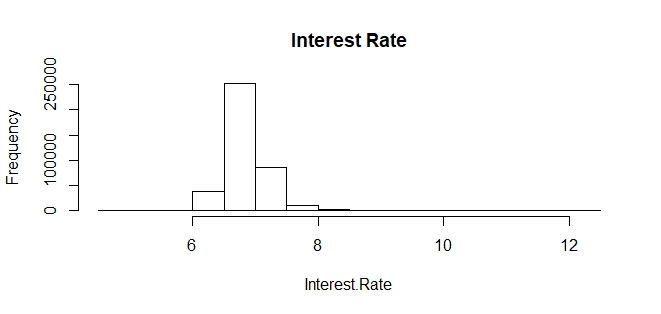
\includegraphics[width=0.45\textwidth]{images/IRB.jpeg}
	\caption{Histogram of Interest Rate}
	\label{fig:IRB}
\end{figure}

%PT
\begin{figure}
	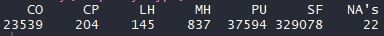
\includegraphics[width=0.45\textwidth]{images/PTS.JPG}
	\caption{Summary Statistics of Property Type}
	\label{fig:PTS}
\end{figure}
\begin{figure}
	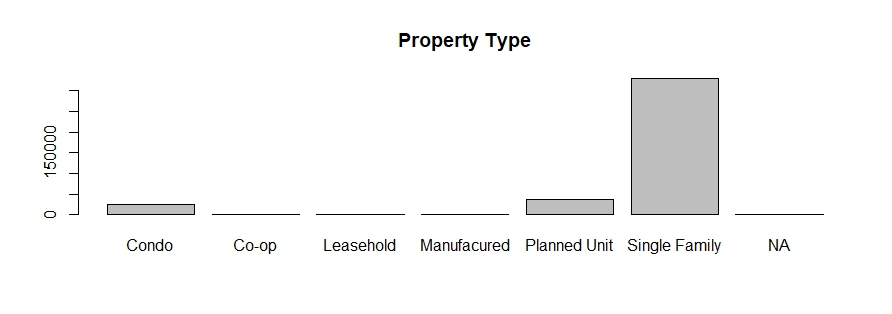
\includegraphics[width=0.45\textwidth]{images/PTB.jpeg}
	\caption{Bar Chart of Property Type}
	\label{fig:PTB}
\end{figure}

%NOB
\begin{figure}
	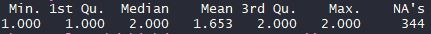
\includegraphics[width=0.45\textwidth]{images/NOBS.JPG}
	\caption{Summary Statistics of Number of Borrowers}
	\label{fig:NOBS}
\end{figure}
\begin{figure}
	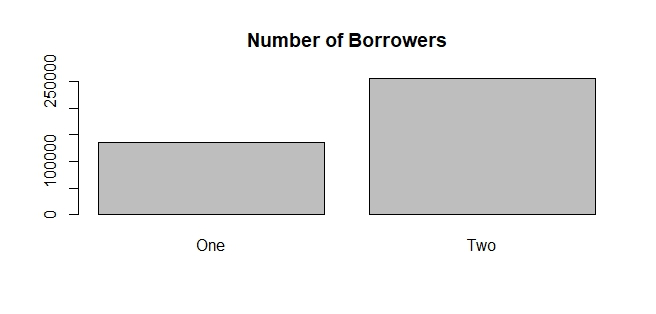
\includegraphics[width=0.45\textwidth]{images/NOBB.jpeg}
	\caption{Bar Chart of Number of Borrowers}
	\label{fig:NOBB}
\end{figure}

%NPV
\begin{figure}
	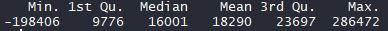
\includegraphics[width=0.45\textwidth]{images/NPVS.JPG}
	\caption{Summary Statistics of Net Present Value}
	\label{fig:NPVS}
\end{figure}
\begin{figure}
	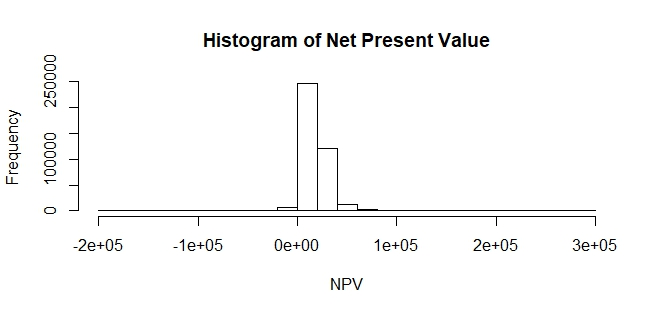
\includegraphics[width=0.45\textwidth]{images/NPVB.jpeg}
	\caption{Histogram of Net Present Value}
	\label{fig:NPVB}
\end{figure}

%Project 2 Figures

\begin{figure}
	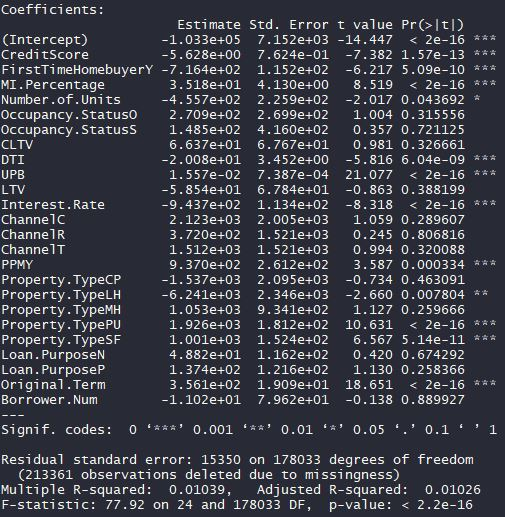
\includegraphics[width=0.45\textwidth]{images/lm1s.jpg}
	\caption{Summary from simple linear regression}
	\label{fig:lm1s}
\end{figure}

\begin{figure}
	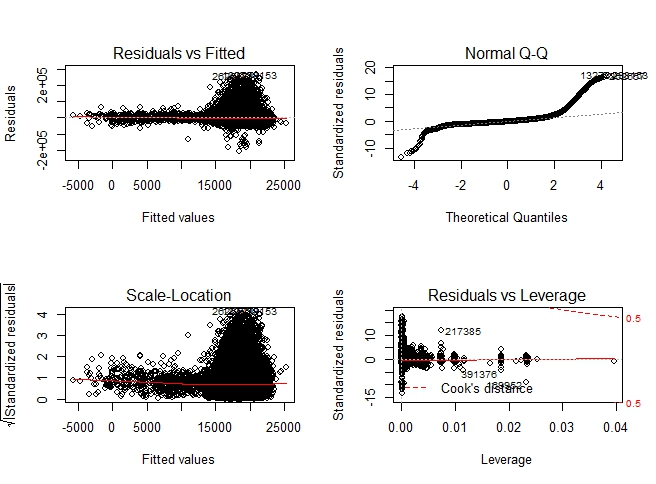
\includegraphics[width=0.45\textwidth]{images/lm1.jpeg}
	\caption{Residual plots of simple linear regression}
	\label{fig:lm1c}
\end{figure}



\begin{figure}
	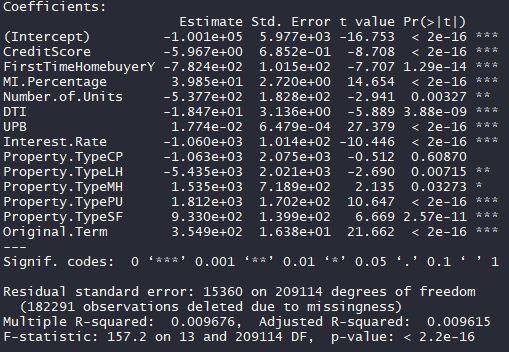
\includegraphics[width=0.45\textwidth]{images/lm2s.jpg}
	\caption{Summary from regression after variable reduction}
	\label{fig:lm2s}
\end{figure}

\begin{figure}
	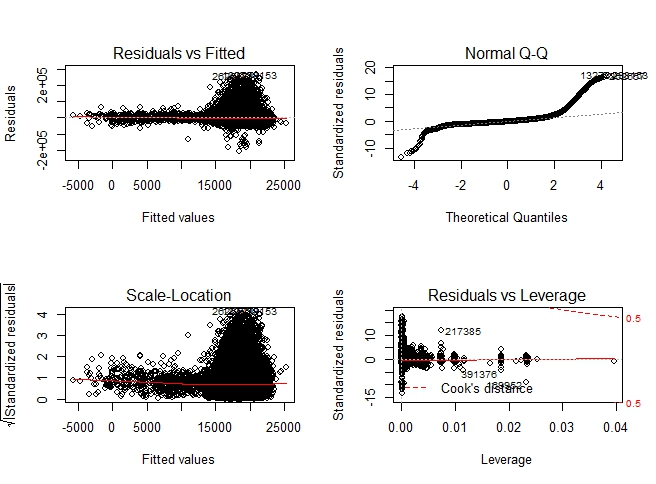
\includegraphics[width=0.45\textwidth]{images/lm1.jpeg}
	\caption{Residual plots after variable reduction}
	\label{fig:lm2c}
\end{figure}

\begin{figure}
	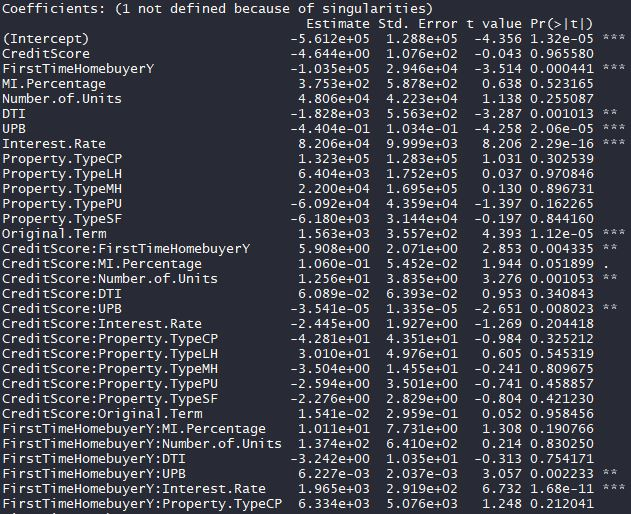
\includegraphics[width=0.45\textwidth]{images/lm3s.jpg}
	\caption{Head of the summary of regression with interactions}
	\label{fig:lm3s}
\end{figure}

\begin{figure}
	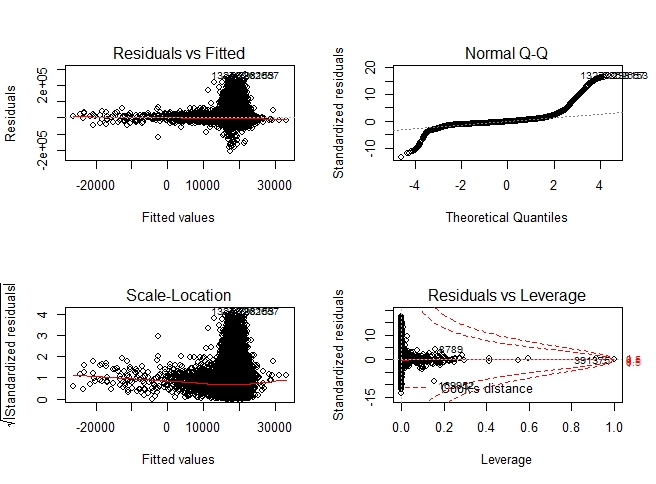
\includegraphics[width=0.45\textwidth]{images/lm3.jpeg}
	\caption{Residual plots with interaction terms}
	\label{fig:lm3c}
\end{figure}

%Project 3 Figure

\begin{figure}
	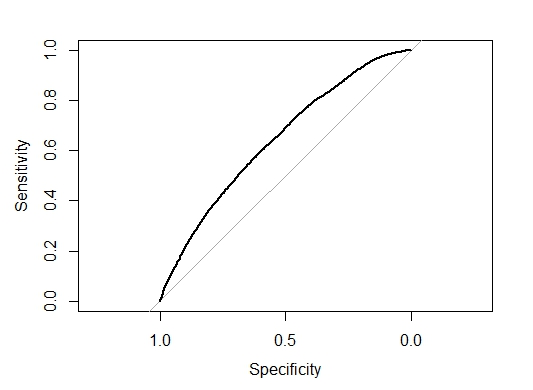
\includegraphics[width=0.45\textwidth]{images/ROC}
	\caption{ROC Curve for Logistic Regression}
	\label{fig:ROC}
\end{figure}


%Project 4 Figures
\begin{figure}
	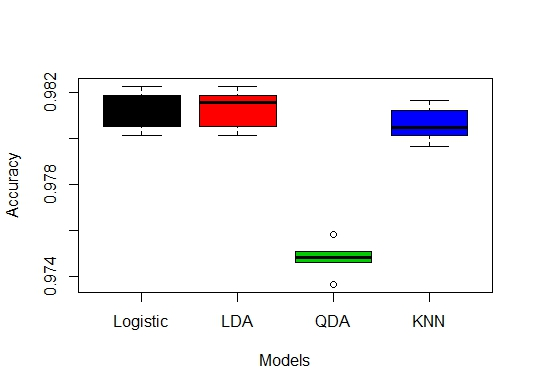
\includegraphics[width=0.45\textwidth]{images/5Fold.jpeg}
	\caption{Accuracies for 5-Fold CV}
	\label{fig:5f}
\end{figure}

%Project 5 Figures
\begin{figure}
	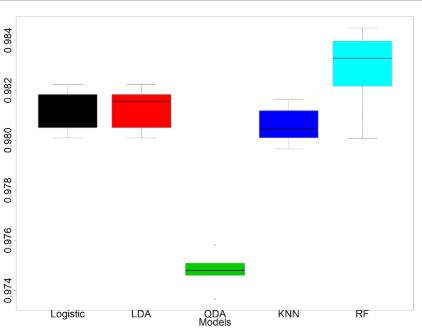
\includegraphics[width=0.45\textwidth]{images/RF.jpg}
	\caption{Accuracies for all 5-Fold CV}
	\label{fig:RF}
\end{figure}

\end{document}
